% Source ID: src-c47985c709ff8ae42e6e192879d604223c58a53c4358056d28f78ad5a9736e3c
% Source PDF SHA-256: a33455d27abdf2c4b344a5b90395bd71269f6fbefdef350375aba074e47ef700
% Source page 2 (printed page 944), question 18. Axes, ellipse, secant, and point G follow the fixed page.
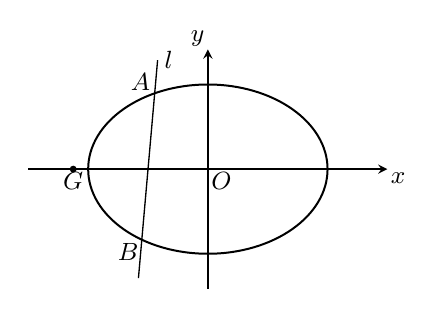
\begin{tikzpicture}[
  x=0.76cm,
  y=0.76cm,
  >=stealth,
  every node/.style={font=\small,inner sep=1pt},
  line width=0.48pt
]
\draw[line width=0.72pt] (0,0) ellipse [x radius=2,y radius=1.4142];
\draw[->] (-3.0,0)--(3.0,0) node[below right] {$x$};
\draw[->] (0,-2.0)--(0,2.0) node[above left] {$y$};
\draw (-1.16,-1.82)--(-0.84,1.82);
\fill (-2.25,0) circle (1.25pt);

\node[above left] at (-0.91,1.26) {$A$};
\node[below left] at (-1.10,-1.18) {$B$};
\node[above right] at (-0.78,1.62) {$l$};
\node[below right] at (0,0) {$O$};
\node[below] at (-2.25,0) {$G$};
\end{tikzpicture}
